\newpage
\section*{{\Large 문제 B.} \tabto{2cm}{\LARGE 2023 아주머학교 프로그래딩 정시머힌}}

\begin{itemize}
    \item 시간 제한 \tabto{2cm} 1초
\end{itemize}

\hrule

\subsection*{문제}

2023 APC를 총괄하고 있는 A.N.S.I 부회장 현빈이는 문제들을 검수하던 중 이상한 점을 발견하였다. 그것은 몇몇 단어들이 비슷하게 생겼지만, 다른 철자로 되어있었던 것이었다. 어리둥절한 현빈이는 누가 이러한 짓을 저질렀는지 고민하던 와중, 어제 선우와 했던 대화가 문득 떠올랐다.

\begin{figure}[h]
    \centering
    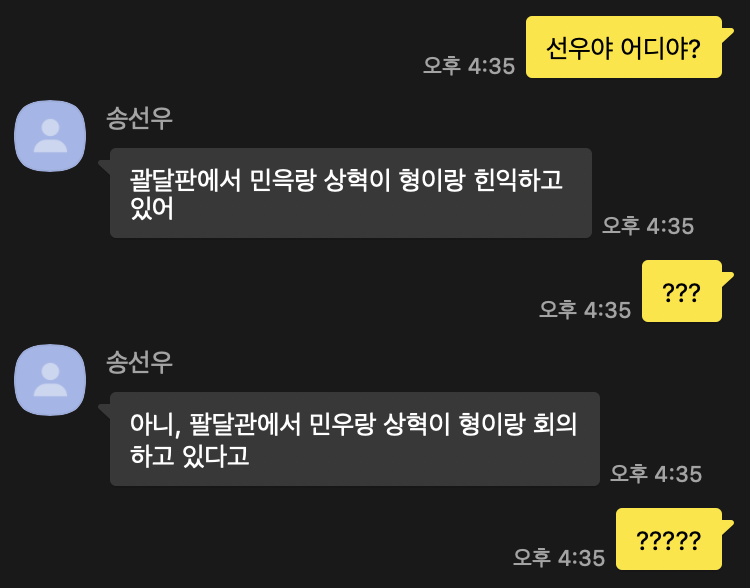
\includegraphics[width=0.4\textwidth]{problems/image/yamin.png}
    \caption{[그림 1] 실제 대화 내용이다.}
\end{figure}

가뜩이나 A.N.S.I 부회장으로서 바쁜 현빈이는 철자가 바뀐 단어들을 다시 원래대로 고치기가 매우 귀찮았다. 다행히도 현빈이는 평소 선우가 어떠한 철자를 바꾸는지 알고 있다. 선우는 알파벳 소문자에 대해서만 철자를 바꾸며, 목록은 다음과 같다.

\begin{table}[h]
\centering
\renewcommand{\arraystretch}{1.5}
\begin{tabular}{|L{2.5cm}|L{2.5cm}|}
\hline
\multicolumn{1}{|c|}{\textbf{원본}} & \multicolumn{1}{c|}{\textbf{수정본}} \\ \hline\hline
\texttt{a} & \texttt{@}\\ \hline
\texttt{c} & \texttt{[}\\ \hline
\texttt{i} & \texttt{!}\\ \hline
\texttt{j} & \texttt{;}\\ \hline
\texttt{n} & \texttt{\^}\\ \hline
\texttt{o} & \texttt{0}\\ \hline
\texttt{t} & \texttt{7}\\ \hline
\texttt{v} & \texttt{\text{\textbackslash'}}\\ \hline
\texttt{w} & \texttt{\text{\textbackslash\textbackslash'}}\\ 
\hline
\end{tabular}
\caption{[표 1] 선우가 바꾸는 철자 목록}
\end{table}

철자가 바뀐 단어들을 보며 어지러웠던 현빈이는 단어에 있는 알파벳의 절반 이상이 바뀌어 있으면 해석을 포기하기로 하였다.

표를 참고하여 현빈이가 주어지는 단어들을 해석할 수 있는지 알아보자.

\newpage

\subsection*{입력}

첫 번째 줄에는 정수 $N$이 주어진다. $(1 \leq N \leq 100)$

두 번째 줄에는 $N$줄에 걸쳐 선우가 바꾸어 놓은 단어들이 주어진다. 선우가 바꾼 단어는 본래 알파벳 소문자로만 구성되어 있었으며, 단어의 길이는 $100$ 이하이다.

\subsection*{출력}

현빈이가 주어진 단어를 해석할 수 있다면 선우가 바꾸기 전의 원래 단어를, 해석을 포기했다면 \texttt{\color{red}I don’t understand}를 $N$줄에 걸쳐 출력한다.

\subsection*{예제}

\begin{table}[h]
% \centering
\renewcommand{\arraystretch}{1.5}
\begin{tabular}{|L{8.2cm}|L{8.2cm}|}
\hline
\multicolumn{1}{|c|}{\textbf{standard input}} & \multicolumn{1}{c|}{\textbf{standard output}} \\ \hline\hline
% 적절한 예제를 입력하면 됩니다.
\texttt{4} & \texttt{ajou}\\ 
\texttt{a;ou} & \texttt{discovery}\\ 
\texttt{d!sc0\textbackslash'ery} & \texttt{kdollar}\\ 
\texttt{kdollar} & \texttt{I don't understand}\\ 
\texttt{\textbackslash'e[70r} & \\

\hline
\end{tabular}
\end{table}

% \newpage

% \vspace*{10cm}
% \begin{center}
%     {\Huge \color{gray} 여백의 미} 
% \end{center}